\citelink{basal}{Basal ganglia is a part of the human brain which is group of subcortical nuclei responsible primarily for motor control, as well as other roles such as motor learning, executive functions and behaviors, and emotions.} \citelink{hunting}{Huntington’s disease is a disorder that causes the progressive degeneration of the basal nuclei.}\par

Hospital de Bellvitge provided an excellent dataset of \ac{MRI} and \ac{dMRI} records. This dataset contains 35 control and 45 Huntington records of already \citelink{register}{registered} T1 \ac{MRI} images with isotropic voxels of 1 millimeter resolution and \ac{dMRI} images with isotropic voxels of 2 millimeter resolution and 1 second temporal resolution. Furthermore this dataset also contains the mask for the basal ganglia, which will also be referenced as the \ac{ROI}. And taking inspiration from this \citelink{conn}{paper}, masks for the 7 main cortical regions of the brain, which will also be referenced as the target regions: limbic, executive, rostral-motor, caudal-motor, parietal, occipital and temporal are also included in the dataset. Tractography was performed on the \ac{dMRI} images to figure out which parts of the \ac{ROI} are connected to which cortical target, in a similar manner to how it was done in said \citelink{conn}{paper}; where the connectivity maps are representing the probability of connections with each cortical target, which were thresholded at the 50th percentile to minimize overlapping voxels between each segment of the \ac{ROI}.\par

\begin{figure}[H]
\centering
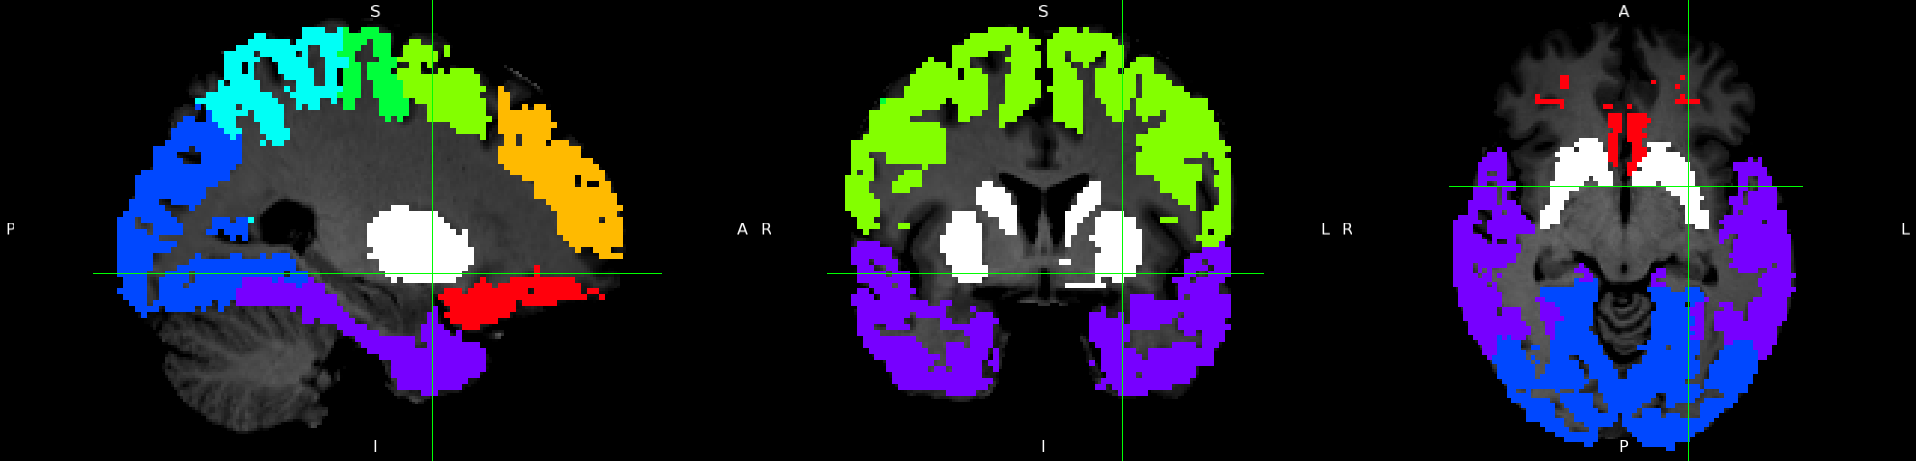
\includegraphics[width=1\textwidth]{rois}
\caption{Basal Ganglia (ROI) \& Cortical Targets}
\label{fig:rois}
\end{figure}

\begin{table}[H]
\centering
\begin{tabular}{|l|l|}
\hline
\textbf{Color} & \textbf{Region} \\ \hline
\begin{tikzpicture}\filldraw[draw=black,fill={rgb,255:red,255;green,255;blue,255}](0,0.15)rectangle(0.25,0.4);\end{tikzpicture} White & Basal Ganglia (ROI) \\ \hline

\begin{tikzpicture}\filldraw[draw=black,fill={rgb,255:red,0;green,255;blue,15}](0,0.15)rectangle(0.25,0.4);\end{tikzpicture} Green & Limbic \\ \hline

\begin{tikzpicture}\filldraw[draw=black,fill={rgb,255:red,255;green,201;blue,126}](0,0.15)rectangle(0.25,0.4);\end{tikzpicture} Brown & Executive \\ \hline

\begin{tikzpicture}\filldraw[draw=black,fill={rgb,255:red,0;green,252;blue,255}](0,0.15)rectangle(0.25,0.4);\end{tikzpicture} Light Blue & Rostral-Motor \\ \hline

\begin{tikzpicture}\filldraw[draw=black,fill={rgb,255:red,251;green,3;blue,255}](0,0.15)rectangle(0.25,0.4);\end{tikzpicture} Purple & Caudal-Motor \\ \hline

\begin{tikzpicture}\filldraw[draw=black,fill={rgb,255:red,253;green,0;blue,0}](0,0.15)rectangle(0.25,0.4);\end{tikzpicture} Red & Parietal \\ \hline

\begin{tikzpicture}\filldraw[draw=black,fill={rgb,255:red,0;green,0;blue,253}](0,0.15)rectangle(0.25,0.4);\end{tikzpicture} Blue & Occipital \\ \hline

\begin{tikzpicture}\filldraw[draw=black,fill={rgb,255:red,255;green,252;blue,0}](0,0.15)rectangle(0.25,0.4);\end{tikzpicture} Yellow & Temporal \\ \hline
\end{tabular}
\caption{Regions Legend}
\label{tab:reglen}
\end{table}

Furthermore, for both the \ac{ROI} and cortical targets, the dataset distinguishes between the right and left halves of the brain. Thus there are actually 2 \ac{ROI}s and $2 \cdot 7=14$ target regions.

\begin{figure}[H]
\centering
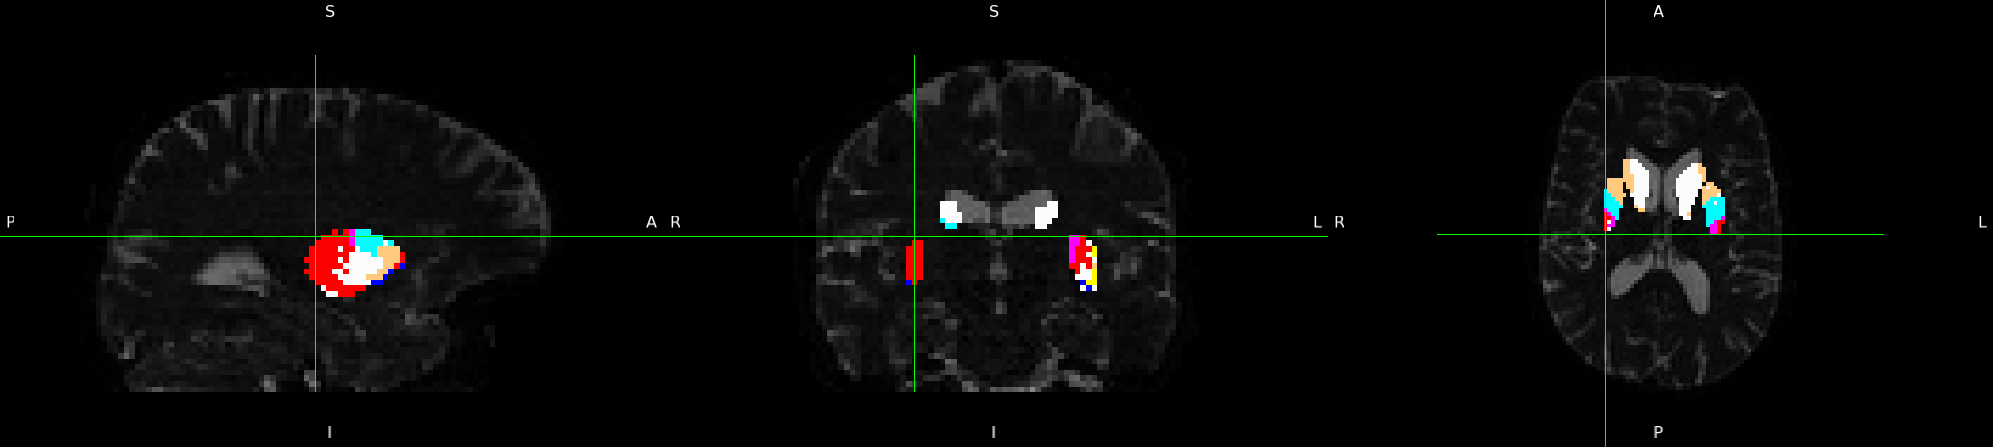
\includegraphics[width=1\textwidth]{conn}
\caption{Connectivity Maps}
\label{fig:conn}
\end{figure}

The goal is to extract the connectivity maps from the T1 \ac{MRI} images, skipping the time and resource consuming process performing \ac{dMRI} and tractorgraphy. Two approaches will be performed in this thesis, trying to extract the connectivity maps from \citelink{radio}{radiomic} features, and trying to extract the connectivity maps with a \ac{FCNN}.\par

All provided files in the dataset are in \ac{NIfTI} format. And all of them are registered in the same anatomical space.\par